\section{The bi-octonions}
\label{sec:bioct}

\subsection{Quaternions and bi-quaternions}

The quaternions $\mathbb H$ are the real combinations of four units $\mathbf e_0=1$, $\mathbf e_1$,
$\mathbf e_2$, $\mathbf e_3$ with the associative product
\begin{equation}
\mathbf e_j^2=-\mathbf e_0,\qquad \mathbf e_1\mathbf e_2=-\mathbf e_2\mathbf e_1=\mathbf e_3
\label{eq:quat}
\end{equation}
and its cyclic permutations ($\mathbf e_2\mathbf e_3=\mathbf e_1$, $\mathbf e_3\mathbf e_1=\mathbf e_2$).
Allowing complex coefficients gives the \emph{bi-quaternions} $\mathbb C\otimes\mathbb H$, whose
elements we write $\mathbf a$, $\mathbf b$, $\mathbf c$, $\mathbf d$. The imaginary unit $i$ of the
coefficients commutes with the units; it is not one of them. The map $M_{\rm LL}$ with
$M_{\rm LL}(\mathbf e_0)=\sigma^{\rm LL}_0$ and $M_{\rm LL}(\mathbf e_j)=-i\sigma^{\rm LL}_j$ (the
Pauli matrices, $j=1,2,3$), extended complex-linearly, is an isomorphism of $\mathbb C\otimes\mathbb H$
onto the complex $2\times2$ matrices: $M_{\rm LL}(\mathbf a\mathbf b)=M_{\rm LL}(\mathbf a)M_{\rm
LL}(\mathbf b)$. Under it the norm of a bi-quaternion, $N_{\rm LL}(\mathbf b)=\sum_p\xi^{\rm
LL}_p(\mathbf b)^2$ (the sum of the squares of its four complex coefficients, $p=0,\dots,3$), becomes
the determinant, and the unit bi-quaternions become the group $SL(2,\mathbb C)$, the double cover of
the Lorentz group of $3+1$ dimensions.

\subsection{Bi-octonions}

The bi-octonions $\mathbb B_{\rm LL}$, which have been used in particle physics
before~\cite{GunaydinGursey1973,Dixon1994,Okubo1995,Furey2016}, are pairs of bi-quaternions, written
$\mathbf x=\mathbf a+\mathbf b\,\mathbf e_4$, with the Cayley-Dickson product
\begin{equation}
(\mathbf a+\mathbf b\,\mathbf e_4)(\mathbf c+\mathbf d\,\mathbf e_4)=(\mathbf a\mathbf c-\bar{\mathbf d}\mathbf b)+(\mathbf d\mathbf a+\mathbf b\bar{\mathbf c})\,\mathbf e_4 ,
\label{eq:cd}
\end{equation}
where the bar changes the signs of the coefficients of $\mathbf e_1$, $\mathbf e_2$, $\mathbf e_3$. The
eight units are $\mathbf e_0,\dots,\mathbf e_3$, $\mathbf e_4$ and $\mathbf e_5=\mathbf e_1\mathbf e_4$,
$\mathbf e_6=\mathbf e_2\mathbf e_4$, $\mathbf e_7=\mathbf e_3\mathbf e_4$; every bi-octonion is
$\mathbf x=\sum_{p=0}^7\xi^{\rm LL}_p(\mathbf x)\,\mathbf e_p$ with complex coefficients, so
$\mathbb B_{\rm LL}$ has real dimension 16. The real combinations form the octonions $\mathbb O$.
Figure~\ref{fig:tables}(a) shows the product of the units. Three special cases of Eq.~(\ref{eq:cd}) are
used throughout:
\begin{align}
\mathbf a(\mathbf b\,\mathbf e_4)&=(\mathbf b\mathbf a)\,\mathbf e_4,\qquad (\mathbf b\,\mathbf e_4)\mathbf c=(\mathbf b\bar{\mathbf c})\,\mathbf e_4,\nonumber\\
(\mathbf b\,\mathbf e_4)(\mathbf d\,\mathbf e_4)&=-\bar{\mathbf d}\mathbf b .
\label{eq:cdspecial}
\end{align}
The \emph{conjugation} $\bar{\mathbf x}$ changes the signs of the coefficients of
$\mathbf e_1,\dots,\mathbf e_7$; it is complex-linear and reverses products,
$\overline{\mathbf x\mathbf y}=\bar{\mathbf y}\bar{\mathbf x}$. The complex conjugation $\mathbf x^*$
conjugates every coefficient, and $\mathbf x^\dagger=(\bar{\mathbf x})^*$. The \emph{norm}
$N_{\rm LL}(\mathbf x)=\sum_p\xi^{\rm LL}_p(\mathbf x)^2$ is a complex number with
$\mathbf x\bar{\mathbf x}=N_{\rm LL}(\mathbf x)\,\mathbf e_0$; its polarization is
$N_{\rm LL}(\mathbf x,\mathbf y)=\sum_p\xi^{\rm LL}_p(\mathbf x)\xi^{\rm LL}_p(\mathbf y)$.

\begin{figure*}[t]
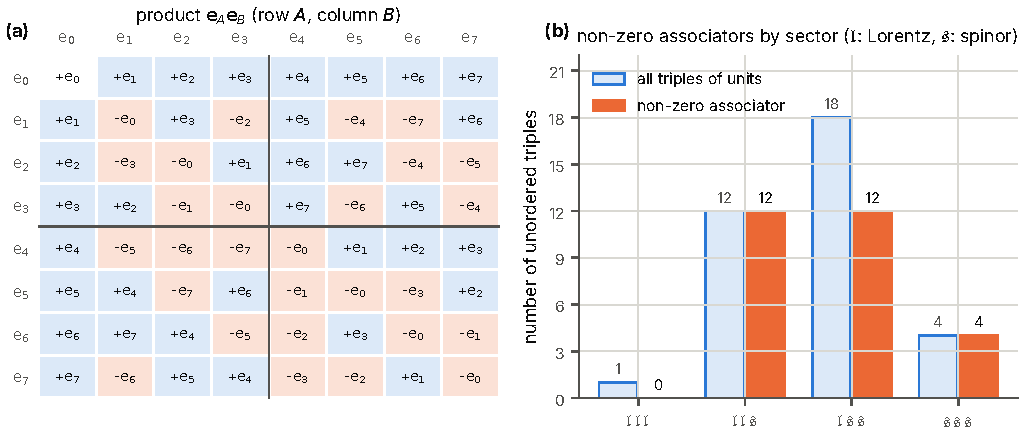
\includegraphics[width=\textwidth]{../figures/fig_sl_tables.pdf}
\caption{(a) The product $\mathbf e_p\mathbf e_{p'}$ of the units of $\mathbb B_{\rm LL}$ (row: left
factor; column: right factor; orange: a minus sign), from Eq.~(\ref{eq:cd}); the lines separate the
quaternion units $\mathbf e_0,\dots,\mathbf e_3$ from $\mathbf e_4,\dots,\mathbf e_7$. (b) The
unordered triples of distinct imaginary units, sorted by how many lie in the Lorentz part
$\mathfrak l_{\rm LL}$ (units $\mathbf e_1$, $\mathbf e_2$, $\mathbf e_3$) and how many in the spinor
charges $\mathfrak s_{\rm LL}$ (units $\mathbf e_4,\dots,\mathbf e_7$), and the number with a non-zero
associator: {{GEN:assoc_nonzero}} ordered triples of units in all (check A-2).}
\label{fig:tables}
\end{figure*}

\subsection{Alternative, not associative}

The \emph{associator} $[\mathbf x,\mathbf y,\mathbf z]=(\mathbf x\mathbf y)\mathbf z-\mathbf x(\mathbf
y\mathbf z)$ measures the failure of associativity. For the bi-octonions:
\begin{enumerate}
\item The norm is multiplicative, $N_{\rm LL}(\mathbf x\mathbf y)=N_{\rm LL}(\mathbf x)N_{\rm LL}(\mathbf
y)$ (check A-3, exact on random bi-octonions with Gaussian-integer coefficients).
\item The associator is \emph{alternating}: it changes sign when two arguments are exchanged, and so
vanishes when two arguments are equal (A-1). An algebra with this property is called
\emph{alternative}; in it any two elements generate an associative subalgebra (Artin's
theorem~\cite{Schafer1966}).
\item The product is not associative: {{GEN:assoc_nonzero}} of the 512 ordered triples of units have
a non-zero associator, the triples of three distinct imaginary units that do not lie in a common
quaternion subalgebra; for example $[\mathbf e_1,\mathbf e_2,\mathbf e_4]=2\mathbf e_7$ (A-2).
Figure~\ref{fig:tables}(b) sorts them.
\item The Moufang identities
$\mathbf z(\mathbf x(\mathbf z\mathbf y))=((\mathbf z\mathbf x)\mathbf z)\mathbf y$,
$((\mathbf y\mathbf z)\mathbf x)\mathbf z=\mathbf y(\mathbf z(\mathbf x\mathbf z))$ and
$(\mathbf z\mathbf x)(\mathbf y\mathbf z)=(\mathbf z(\mathbf x\mathbf y))\mathbf z$ hold (A-3).
\end{enumerate}
Because the associator is alternating, the six associators of Eq.~(\ref{eq:jacassoc}) are all equal
up to their signs, and the Jacobiator of the commutator is
\begin{equation}
\mathrm{Jac}_{\rm LL}(\mathbf x,\mathbf y,\mathbf z)=6\,[\mathbf x,\mathbf y,\mathbf z]
\label{eq:jac6}
\end{equation}
(A-4): the Jacobi identity fails exactly where associativity fails.

\subsection{The super-loop and its Malcev algebra}

A \emph{loop} is a set with a product, an identity element, and unique solutions of the equations
$\mathbf w\mathbf x=\mathbf y$ and $\mathbf x\mathbf w=\mathbf y$ for $\mathbf x$; a group is an
associative loop. A \emph{Moufang loop} obeys the Moufang identities~\cite{Moufang1935}. The unit
bi-octonions
\begin{equation}
\mathbb L_{\rm LL}=\{\mathbf w\in\mathbb B_{\rm LL}:\ N_{\rm LL}(\mathbf w)=1\}
\label{eq:loop}
\end{equation}
form a Moufang loop: the product of two of them is one of them (the norm is multiplicative), $\mathbf
e_0$ is the identity, $\bar{\mathbf w}$ is the inverse of $\mathbf w$, and $\mathbf w\mathbf x=\mathbf y$
has the unique solution $\mathbf x=\bar{\mathbf w}\mathbf y$, because $\bar{\mathbf w}(\mathbf w\mathbf
y)=(\bar{\mathbf w}\mathbf w)\mathbf y$ by alternativity. We call it the \emph{Lorentz super-loop}. It
is a complex manifold of complex dimension 7 (real dimension 14), and it contains $SL(2,\mathbb C)$,
the unit bi-quaternions, as a subgroup.

Just as a Lie group has a Lie algebra, a Moufang loop that is a smooth manifold has a tangent algebra
at the identity: the imaginary bi-octonions $\mathfrak m_{\rm LL}=\mathbb C\otimes{\rm Im}\,\mathbb O$
with the commutator (real dimension 14). It is not a Lie algebra, by Eq.~(\ref{eq:jac6}), but it is a
\emph{Malcev algebra}~\cite{Malcev1955,Sagle1961}: its bracket is bilinear and antisymmetric and obeys
the Malcev identity $\mathrm{Jac}_{\rm LL}(\mathbf x,\mathbf y,[\mathbf x,\mathbf z])=[\mathrm{Jac}_{\rm
LL}(\mathbf x,\mathbf y,\mathbf z),\mathbf x]$, which in a Lie algebra holds trivially. We verify it in
the linearized form, obtained by replacing $\mathbf x$ by $\mathbf x+\mathbf w$ and keeping the part
linear in $\mathbf w$,
\begin{align}
&\mathrm{Jac}_{\rm LL}(\mathbf x,\mathbf y,[\mathbf w,\mathbf z])+\mathrm{Jac}_{\rm LL}(\mathbf w,\mathbf y,[\mathbf x,\mathbf z])\nonumber\\
&\quad=[\mathrm{Jac}_{\rm LL}(\mathbf x,\mathbf y,\mathbf z),\mathbf w]+[\mathrm{Jac}_{\rm LL}(\mathbf w,\mathbf y,\mathbf z),\mathbf x],
\label{eq:malcev}
\end{align}
on all 2401 4-tuples of imaginary units (A-5). Malcev algebras are to analytic Moufang loops what Lie
algebras are to Lie groups~\cite{Malcev1955,Kuzmin1971,NagyStrambach2002}.

\subsection{No realization by operators}

\noindent\emph{Theorem R.} (a) Every linear map $\varrho_{\rm LL}$ from $\mathfrak m_{\rm LL}$ to the
linear operators on a vector space that turns brackets into commutators,
$\varrho_{\rm LL}([\mathbf x,\mathbf y])=\varrho_{\rm LL}(\mathbf x)\varrho_{\rm LL}(\mathbf
y)-\varrho_{\rm LL}(\mathbf y)\varrho_{\rm LL}(\mathbf x)$, is zero. (b) No one-to-one map of
$\mathbb L_{\rm LL}$ into the invertible operators on a vector space turns the product of the loop into
the product of operators.

\noindent\emph{Proof.} (a) Applying $\varrho_{\rm LL}$ to Eq.~(\ref{eq:jacobiator}) gives
$\varrho_{\rm LL}(\mathrm{Jac}_{\rm LL}(\mathbf x,\mathbf y,\mathbf z))=\mathrm{Jac}_{\rm
LL}(\varrho_{\rm LL}(\mathbf x),\varrho_{\rm LL}(\mathbf y),\varrho_{\rm LL}(\mathbf z))$, and the right
side vanishes by Eq.~(\ref{eq:jacassoc}), because the product of operators is associative (A-6). Hence
$\varrho_{\rm LL}$ vanishes on every Jacobiator. The Jacobiators of the real basis $\mathbf e_p$,
$i\mathbf e_p$ ($p=1,\dots,7$) of $\mathfrak m_{\rm LL}$ span a space of real dimension
{{GEN:jac_rank}}, all of $\mathfrak m_{\rm LL}$ (A-8); so $\varrho_{\rm LL}=0$. (b) Such a map would
send $(\mathbf e_1\mathbf e_2)\mathbf e_4=\mathbf e_7$ and $\mathbf e_1(\mathbf e_2\mathbf e_4)=-\mathbf
e_7$ to the same operator, because both products of operators are equal; it would not be one-to-one.
$\square$

In particular the left multiplications $L^{\rm LL}_{\mathbf x}:\mathbf y\mapsto\mathbf x\mathbf y$, real
$16\times16$ matrices, do not represent $\mathfrak m_{\rm LL}$: $[L^{\rm LL}_{\mathbf e_1},L^{\rm
LL}_{\mathbf e_4}]\neq L^{\rm LL}_{[\mathbf e_1,\mathbf e_4]}$ (A-7). Theorem R is the precise sense in
which the non-associativity is essential: no reformulation by operators, and so no Hilbert space of
states on which the super-loop acts linearly and faithfully, removes it. Hypotheses H-grp, H-op and
H-Lie fail for $\mathbb L_{\rm LL}$, and they fail together.
